\documentclass{beamer}

\usepackage[utf8]{inputenc}

\usetheme{Madrid}
\setbeamerfont{normal text}{size=\small}

\usecolortheme{default}
\usepackage{extarrows}
\usepackage{amsmath}
\usepackage{extarrows}
\usepackage{amssymb,amsfonts,amsthm}
\usepackage{txfonts}
\usepackage{tkz-euclide}
\usepackage{listings}
\usepackage{adjustbox}
\usepackage{array}
\usepackage{tabularx}
\usepackage{gvv}
\usepackage{lmodern}
\usepackage{circuitikz}
\usepackage{tikz}
\usepackage{graphicx}
\usepackage{amsmath} 
\usepackage{multicol}

\setbeamertemplate{page number in head/foot}[totalframenumber]

\usepackage{tcolorbox}
\tcbuselibrary{minted,breakable,xparse,skins}

\definecolor{bg}{gray}{0.95}
\DeclareTCBListing{mintedbox}{O{}m!O{}}{%
  breakable=true,
  listing engine=minted,
  listing only,
  minted language=#2,
  minted style=default,
  minted options={%
    linenos,
    gobble=0,
    breaklines=true,
    breakafter=,,
    fontsize=\small,
    numbersep=8pt,
    #1},
  boxsep=0pt,
  left skip=0pt,
  right skip=0pt,
  left=25pt,
  right=0pt,
  top=3pt,
  bottom=3pt,
  arc=5pt,
  leftrule=0pt,
  rightrule=0pt,
  bottomrule=2pt,
  toprule=2pt,
  colback=bg,
  colframe=orange!70,
  enhanced,
  overlay={%
    \begin{tcbclipinterior}
    \fill[orange!20!white] (frame.south west) rectangle ([xshift=20pt]frame.north west);
    \end{tcbclipinterior}},
  #3,
}
\lstset{
    language=C,
    basicstyle=\ttfamily\small,
    keywordstyle=\color{blue},
    stringstyle=\color{orange},
    commentstyle=\color{green!60!black},
    numbers=left,
    numberstyle=\tiny\color{gray},
    breaklines=true,
    showstringspaces=false,
}


\title{1.1.32 - Analog Signal Processing }
\author{Kartik Lahoti : EE25BTECH11032}

\begin{document}

\begin{frame}
    \titlepage
\end{frame}

\begin{frame}
    \section{Question}
    \quad If $x = \text{Re}\ G(j\omega)$, and $y = \text{Im}\ G(j\omega)$ then for $\omega \to 0^{+}$, the Nyquist plot for
$$G(s) = \frac{1}{s(s+1)(s+2)}$$ 
becomes asymptotic to the line\hfill{(EE 2007)} 
    \begin{multicols}{4}
        \begin{enumerate}
        \item  $x = 0$
        \item  $x = -3/4$
        \item  $x = y - 1/6$
        \item  $x = y/\sqrt{3}$
        \end{enumerate}
    \end{multicols}
\end{frame}

\begin{frame}
    \frametitle{Theory}\\
    $G(s)$ represents the open-loop transfer function of a system in the Laplace domain.
    \begin{figure}
        \centering
        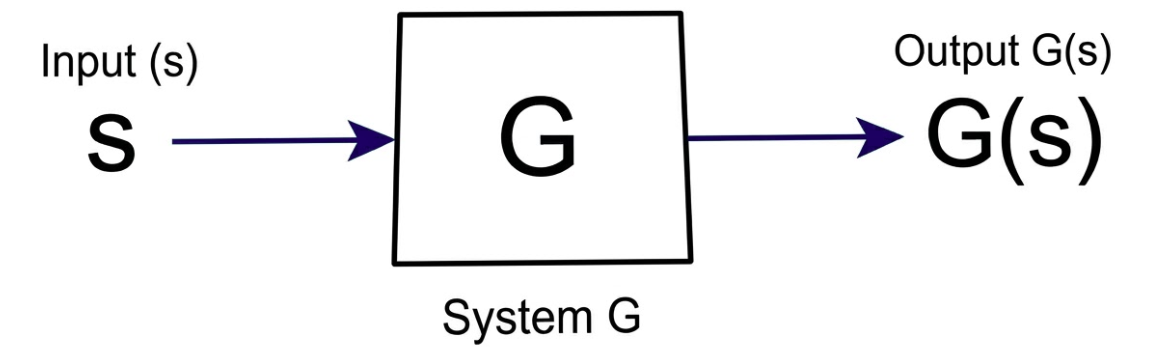
\includegraphics[width=0.75\columnwidth]{figs/fig1.png}
        \caption{Function $G(s)$}
        \label{fig:fig1}
    \end{figure}
    \begin{align}
        G(s) = \frac{1}{s(s+1)(s+2)}
    \end{align}
\end{frame}

\begin{frame}
    \frametitle{Transfer Function}\\
    When analyzing linear, time-invariant (LTI) systems in analog signal processing, working with differential equations in the time domain can get incredibly messy.By applying the Laplace transform (assuming all initial conditions are zero), we move from the time domain to the $s$-domain.
    \begin{align}
        G(s) = \frac{\mathcal{L}\{\text{Output}\}}{\mathcal{L}\{\text{Input}\}}
    \end{align}

\end{frame}

\begin{frame}
    \frametitle{Poles of System}
    From:
    \begin{align}
        s(s+1)(s+2) = 0 
    \end{align}
    Poles are at :
    \begin{itemize}
        \item $s = 0$
        \item $s = -1$
        \item $s = -2$ 
    \end{itemize}
\end{frame}

\begin{frame}
    \frametitle{Solution}
    Rewriting: 
    \begin{align}
        G(s) = \frac{1}{s}\cdot\frac{1}{\brak{s+1}\brak{s+2}}
    \end{align}

    \begin{itemize}
        \item $\frac{1}{s} \rightarrow $ integrator
        \item $\frac{1}{(s+1)(s+2)}  \rightarrow $ finite gain without discontinuity
    \end{itemize}

\end{frame}

\begin{frame}
\frametitle{Interpretation of Each Block}

\textbf{Integrator:} $\frac{1}{s} = \frac{1}{j\omega}$
\begin{itemize}
    \item Magnitude tends to infinity as $\omega \to 0$
    \item Phase is $-90^\circ$
    \item Hence, the Nyquist plot is directed vertically downward near the origin
\end{itemize}

\vspace{0.5cm}

\textbf{Remaining Block:}
\begin{align}
    H(j\omega) = \frac{1}{(1 + j\omega)(2 + j\omega)}
\end{align}

At low frequencies ($\omega \to 0$):
\begin{itemize}
    \item The system behaves as a constant gain element
    \item Evaluating at $\omega = 0$:
\end{itemize}

\begin{align}
    H(0) = \frac{1}{(1)(2)} = \frac{1}{2}
\end{align}

\end{frame}

\begin{frame}
\frametitle{First-Order Approximation (Proof)}

Given:
\begin{align}
H(j\omega) = \frac{1}{(1 + j\omega)(2 + j\omega)}
\end{align}

Expand the denominator:
\begin{align}
(1 + j\omega)(2 + j\omega) &= 2 + 3j\omega + (j\omega)^2 \\
&= 2 + 3j\omega - \omega^2
\end{align}

For $\omega \to 0$, neglect higher-order terms:
\begin{align}
(1 + j\omega)(2 + j\omega) \approx 2 + 3j\omega
\end{align}

Hence,
\begin{align}
H(j\omega) \approx \frac{1}{2 + 3j\omega}
\end{align}
\end{frame}
\begin{frame}
    
Factor out 2:
\begin{align}
H(j\omega) &= \frac{1}{2\brak{1 + \frac{3}{2}j\omega}} \\
&= \frac{1}{2} \cdot \frac{1}{1 + \frac{3}{2}j\omega}
\end{align}

Using the first-order approximation:
\begin{align}
\frac{1}{1 + x} \approx 1 - x \quad \text{for } |x| \ll 1
\end{align}

Let $x = \frac{3}{2}j\omega$, then:
\begin{align}
H(j\omega) &\approx \frac{1}{2} \brak{1 - \frac{3}{2}j\omega} \\
&= \frac{1}{2} - j\frac{3}{4}\omega
\end{align}

\end{frame}

\begin{frame}
    $\therefore$
    \begin{align}
        G(j\omega) = \frac{1}{j\omega}\cdot\brak{\frac{1}{2} - j\frac{3}{4}\omega}
    \end{align}
    Hence, 
    \begin{align}
        x = \text{Re}\ G(j\omega) =  \frac{-3}{4} \text{ and } y = \text{Im}\ G(j\omega) = \frac{-1}{2\omega}
    \end{align}

    Final Nyquist Behavior 
    \begin{align}
        x = \frac{-3}{4} \text { and }  y \rightarrow -\infty 
    \end{align}
    
\end{frame}

\begin{frame}[fragile]
    \frametitle{Python Code }
    \begin{lstlisting}
import control as ctrl
import matplotlib.pyplot as plt
import numpy as np

num = [1]
den = [1, 3, 2, 0] 

G = ctrl.TransferFunction(num, den)

plt.figure()

ctrl.nyquist_plot(G)

   \end{lstlisting}
\end{frame}
\begin{frame}[fragile]
\frametitle{Python Code }
\begin{lstlisting}
plt.axvline(x=-0.75, color='red', linestyle='--', label='Asymptote')

plt.xlim(-1, 0) 
plt.ylim(-10, 10)

plt.title("Nyquist Plot with Low-Frequency Asymptote")
plt.xlabel("Real Axis")
plt.ylabel("Imaginary Axis")
plt.grid()
plt.legend()
plt.savefig('../figs/plt1.png')
plt.show()
    \end{lstlisting}
\end{frame}


\begin{frame}{Plot}
    \centering
    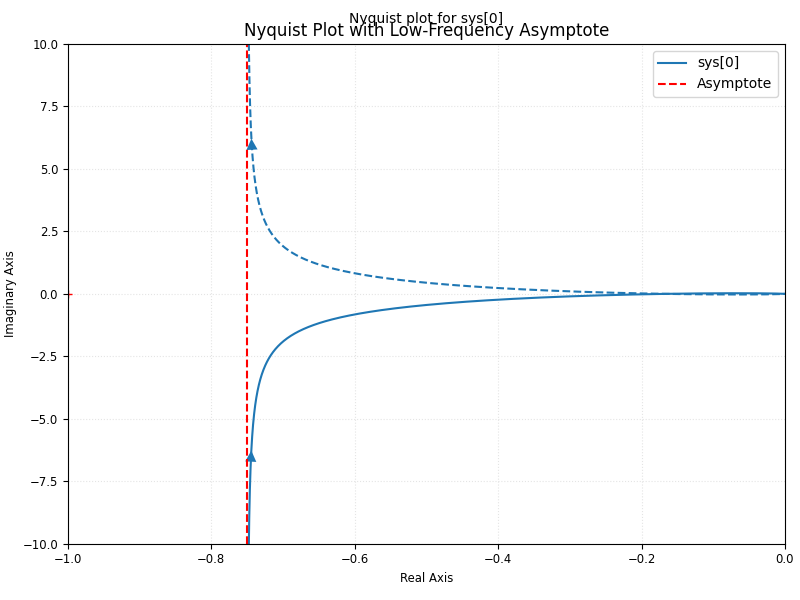
\includegraphics[width=\columnwidth, height=0.8\textheight, keepaspectratio]{figs/plt1.png}   
\end{frame}


\end{document}
